% !TEX encoding = UTF-8
% !TEX TS-program = pdflatex
% !TEX root = ../tesi.tex

%**************************************************************
\chapter{Progettazione e codifica}
\label{cap:progettazione-codifica}
%**************************************************************

\intro{Il capitolo approfondisce l'architettura del software prima complessivamente e poi nel dettaglio, descrivendo i problemi incontrati e la soluzione applicata.}\\

\section{Architettura del modulo}

Il modulo è stato progettato tenendo a mente i requisiti di scalabilità imposti dall'azienda. L'architettura è stata definita durante le prime settimane subendo modifiche, anche in corso d'opera, in risposta ai bisogni ed alle difficoltà rilevate.

\subsection{Master e gestione degli url}

La gestione degli url ha come fulcro una coda celery nella quale vengono immagazzinati gli url da analizzare. Il componente denominato "master" periodicamente inserirà nella coda url estratti da una lista stilata dall'analista. Il modulo "worker" andrà quindi a prelevare gli url dalla coda assicurandosi di non averli già analizzati e tramite essi eseguirà la ricerca di nuovi url. 


\begin{figure}[!h] 
    \centering 
    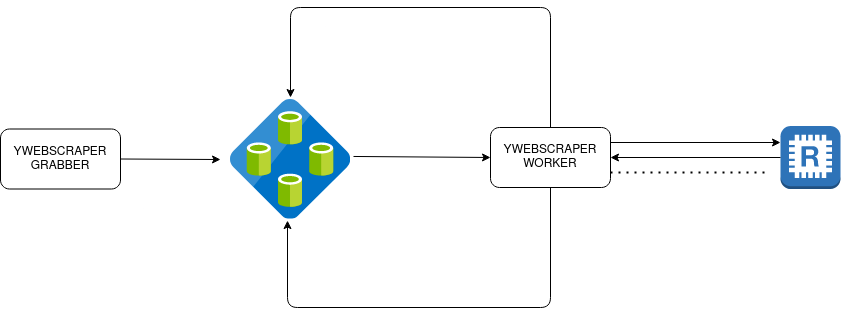
\includegraphics[width=1\columnwidth]{chapter4-project/architettura-gestione-url.png} 
    \caption{Architettura della gestione degli url in dettaglio.}
\end{figure}

\subsubsection{Ricerca nuovi url}

Una delle funzionalità del componente "worker" è l'estrazione degli url dalla coda celery e la loro analisi. Il primo controllo realizzato è se l'url è già stato analizzato, questo viene verificato controllando se è presente o meno nella cache di redis. Se l'url è presente è già stato analizzato, altrimenti deve essere analizzato. Ad inizio analisi l'url viene inserito nella cache redis con un ttl impostato dall'analista. Il worker quindi si occuperà di contattare il sito richiesto utilizzando il metodo specificato dall'analista (requests, celery-chrome, celery-firefox etc) e dal codice sorgente (quindi l'html) andrà ad estrarre e ripulire la lista di url. 


\subsubsection{Pulizia degli url}
Un url (da RFC 1808, Section 2.1 https://datatracker.ietf.org/doc/html/rfc1808.html\#section-2.1) è composto da \newline
<scheme>://<netloc>/<path>;<params>?<query>\#<fragment>
\newline
\begin{itemize}
	\item \textbf{scheme:} indica il protocollo utilizzato;
	\item \textbf{netloc:} \textit{ne}twork \textit{loc}ation, indica il dominio ed i sottodomini (se presenti), il numero di porta e opzionalmente le credenziali con la seguente sintassi: username:password;
	\item \textbf{path:} contiene informazioni sulla specifica risorsa alla quale accedere;
	\item \textbf{params} campo opzionale contenente informazioni aggiuntive sul path, un esempio possono essere le informazioni aggiuntive da portare da una pagina alla successiva;
	\item \textbf{query} campo opzionale contenente informazioni aggiuntive sul path, come da nome questo campo contiene le query;
	\item \textbf{fragment} campo opzionale contenente informazioni aggiuntive sul path, un esempio possono essere i '\#' che indicano in quale parte della risorsa portare la vista.
\end{itemize}

Per realizzare una pulizia degli url completa. serve fare le seguenti operazioni:
\begin{enumerate}
	\item Per evitare di analizzare due pagine identiche con campi fragment differenti, viene eliminato il campo opzionale fragment;
	\item Rendere tutti i caratteri nei campi scheme e netloc minuscoli;
	\item Eliminazione di tutti gli url con contenuto nel campo scheme differente da http o https;
	\item Aggiunta di http nel campo scheme in caso in cui sia vuoto;
	\item Se l'url analizzato è relativo lo si trasforma in url assoluto;
	\item Eliminazione di url uguali all'url iniziale inserito dal modulo "master", all'url precedente e all'url corrente;
	\item Eliminazione degli url presenti nella lista di siti da non esplorare stilata dall'analista.
\end{enumerate}

\subsubsection{Riprovare url}

L'analisi di alcuni url, non andrà sempre a buon fine, per questo è stato necessario progettare una logica solida per riprovare l'analisi. Quando l'analisi di un url fallisce per qualsiasi motivo, esso viene reinserito nella coda contenente gli url da analizzare; all'url verrà assegnata una priorità minore, andando quindi ad inserirlo in fondo alla coda. Viene inoltre modificato il ttl dell'url nella cache di redis, inserendo un ttl minore, in modo che vengano ignorati per un breve lasso di tempo nuovi tentativi con lo stesso url non funzionante, così da non non sovraccaricare il server. Se lo stesso url viene riprovato n volte fallendo, con n scelto dall'analista, allora l'url viene scartato definitivamente.


\subsection{Worker e ricerca di informazioni interessanti}

Il componente denominato "worker" oltre a gestire gli url andrà ad analizzare la pagina alla ricerca di informazioni considerate interessanti.
\begin{figure}[!h] 
    \centering 
    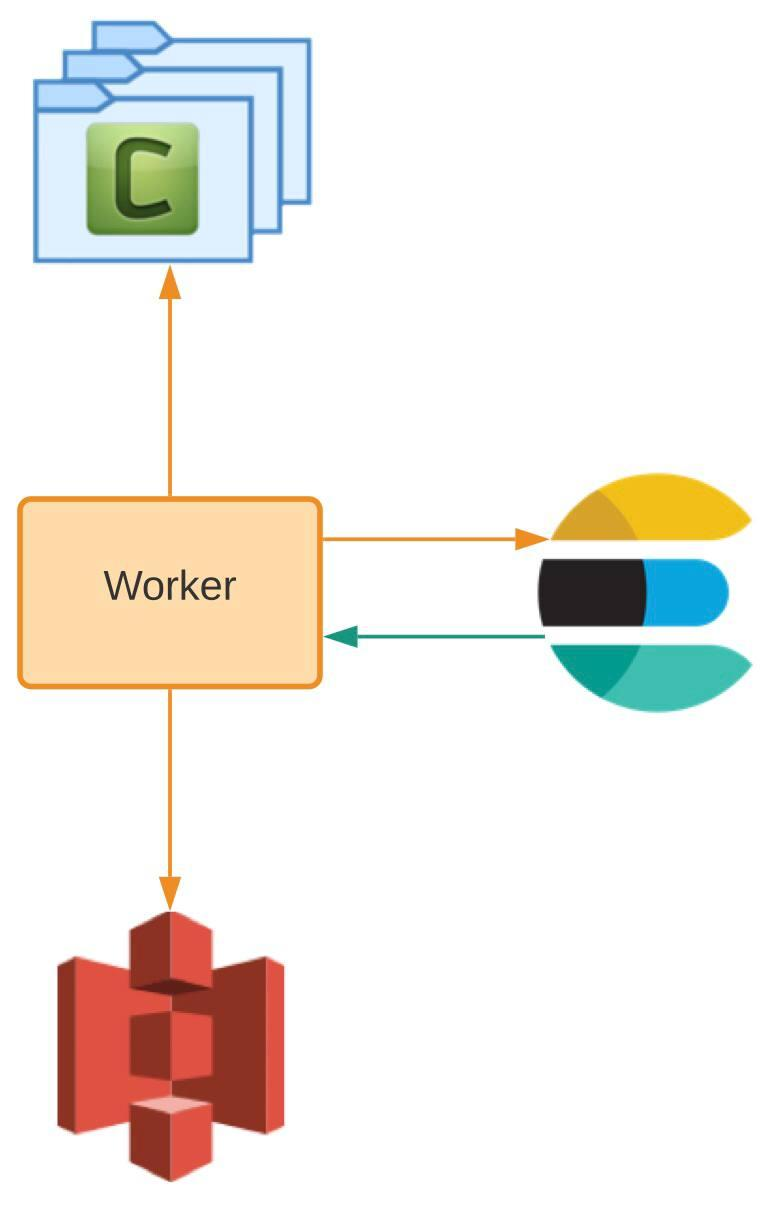
\includegraphics[width=0.4\columnwidth]{chapter4-project/architettura-match-search.png} 
    \caption{Architettura della ricerca di match in dettaglio.}
\end{figure}

\subsubsection{Ricerca informazioni interessanti}

La ricerca di informazioni interessanti avviene ricercando occorrenze sulla pagina html, tramite l'utilizzo di molteplici e complesse regex stese dall'analista in precedenza. Queste regex offrono un grado di granularità aggiuntivo poichè esse vengono sviluppate specificatamente per ogni azienda cliente. Se invece il contenuto del sito non è analizzabile, ad esempio un'immagine, allora viene analizzato l'header restituito dal server. Quando vengono trovate occorrenze in un url si crea l'hash della pagina tramite un algoritmo e viene controllato se l'hash è presente su elasticsearch. Se non è presente allora viene mandato il sito con diverse informazioni aggiuntive nella coda celery. Questa coda è per un modulo differente presente nella infrastruttura, da questa coda infatti le informazioni vengono elaborate e se ritenute valide aggiunte ad Elasticsearch. \newline{}
Se l'hash non è presente su elasticsearch inoltre viene anche salvato il codice sorgente ed una istantanea della pagina su un bucket di Amazon S3.